\section{Modelo de información del registro de la escuela}
Para iniciar con el proceso de acreditación, las escuelas deben registrar sus datos en el sistema. En esta sección se describen todas las entidades relacionadas con el registro de la escuela.

%%================================================================================================	
\subsection{Descripción general}
 En la figura~\ref{fig:registroEscuelas} se muestra la estructura de información que manejará el sistema.
 
\begin{figure}[htbp!]
	\begin{center}
		\fbox{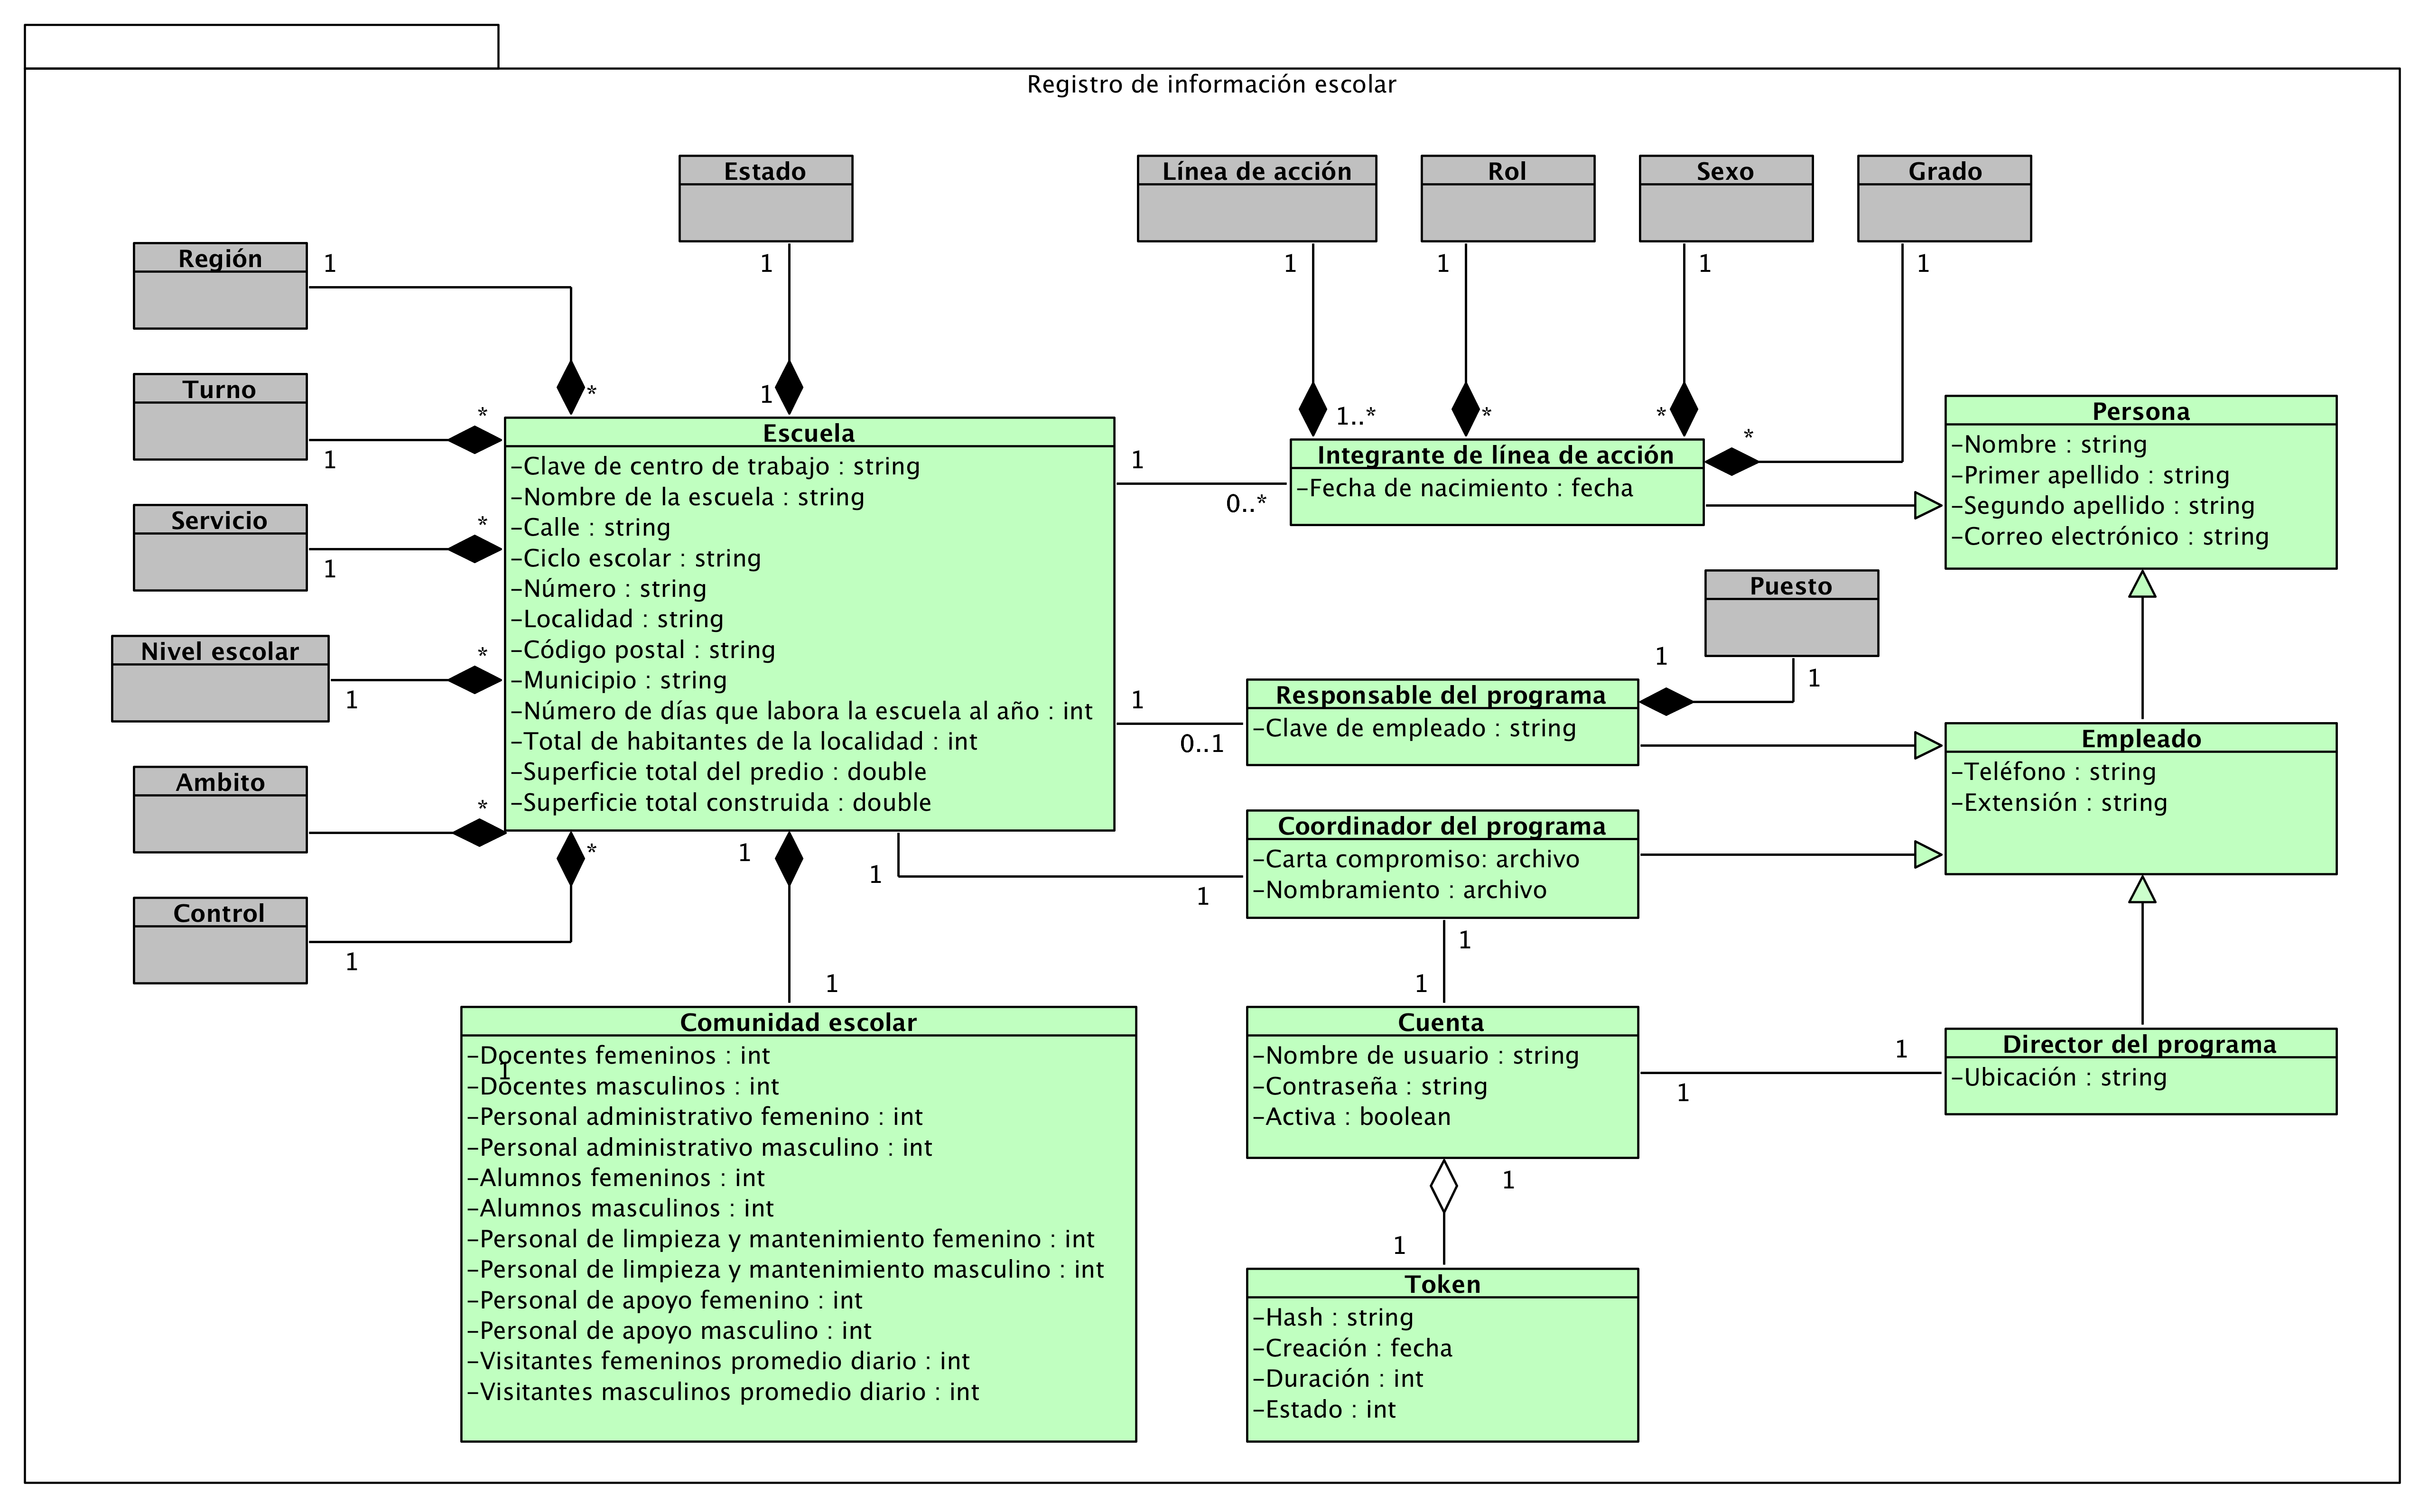
\includegraphics[width=1\textwidth]{images/clases/Registro}}
		\caption{Modelo de información del registro de la escuela}
		\label{fig:registroEscuelas}
	\end{center}
\end{figure}

%----------------------------------------------------------------------------------------------------------------------------------------------------------------
\begin{BusinessEntity}{persona}{Persona}
      \Battr{nombre}{Nombre}{\tdPalabra}{Denominación que se le da a una persona}{\requerido}      
      \Battr{primerApellido}{Primer apellido}{\tdPalabra}{Apellido paterno de una persona}{\requerido}      
      \Battr{segundoApellido}{Segundo apellido}{\tdPalabra}{Apellido materno de una persona}{\requerido}      
      \Battr{correo}{Correo electrónico}{\tdFrase}{Dirección de correo electrónico de una persona}{\opcional}
\end{BusinessEntity}
%----------------------------------------------------------------------------------------------------------------------------------------------------------------
\begin{BusinessEntity}{integrante}{Integrante de línea de acción}
      \Battr{fechaNac}{Fecha de nacimiento}{\tdFecha}{Fecha de nacimiento de un integrante de línea de acción}{\requerido}
      \Battr{lineaAccion}{Línea de acción}{\tdCatalogo}{Es la línea de acción a la que pertenece el integrante}{\requerido}
      \Battr{rol}{Rol}{\tdCatalogo}{Es el \cdtRef{gls:rol}{rol} del integrante}{\requerido}
      \Battr{sexo}{Sexo}{\tdCatalogo}{Es el \cdtRef{gls:sexo}{sexo}del integrante}{\requerido}
      \Battr{grado}{Grado}{\tdCatalogo}{Es el \cdtRef{gls:grado}{grado} del integrante}{\requerido}
\end{BusinessEntity}
  \subsubsection{Relaciones}
  \begin{BusinessFact}{integrante:persona}{Persona}
    \BRitem{Descripción}{Un Integrante de línea de acción es un tipo de \cdtRef{persona}{Persona}}
    \BRitem{Tipo}{\relHerencia}
  \end{BusinessFact}
%----------------------------------------------------------------------------------------------------------------------------------------------------------------
\begin{BusinessEntity}{empleado}{Empleado}
      \Battr{telefono}{Teléfono}{\tdPalabra}{Número telefónico de un empleado, incluyendo la clave lada}{\requerido}      
      \Battr{extension}{Extensión}{\tdPalabra}{Clave que permite la redirección telefónica dentro de una escuela}{\opcional}
\end{BusinessEntity}
  \subsubsection{Relaciones}
  \begin{BusinessFact}{empleado:persona}{Persona}
    \BRitem{Descripción}{Un Empleado es un tipo de \cdtRef{persona}{Persona}}
    \BRitem{Tipo}{\relHerencia}
  \end{BusinessFact}
%----------------------------------------------------------------------------------------------------------------------------------------------------------------
\begin{BusinessEntity}{responsable}{Responsable del programa}
      \Battr{cveEmpleado}{Clave de empleado}{\tdPalabra}{Conjunto de caracteres que identifica a cada empleado dentro de la escuela}{\requerido}
      \Battr{puesto}{Puesto}{\tdCatalogo}{Es el \cdtRef{gls:puesto}{puesto} del responsable del programa}{\requerido}
\end{BusinessEntity}
  \subsubsection{Relaciones}
  \begin{BusinessFact}{responsable:empleado}{Empleado}
    \BRitem{Descripción}{Un Responsable del programa es un tipo de \cdtRef{empleado}{Empleado}}
    \BRitem{Tipo}{\relHerencia}
  \end{BusinessFact}
%----------------------------------------------------------------------------------------------------------------------------------------------------------------
\begin{BusinessEntity}{coordinador}{Coordinador del programa}
       \Battr{cartaCompromiso}{Carta compromiso}{\tdArchivo}{Es el documento que avala el compromiso que una escuela tiene para concluir el programa de acreditación}{\requerido}
       \Battr{nombramiento}{Nombramiento}{\tdArchivo}{Es el documento que avala a una persona como el director actual de una escuela}{\requerido}
\end{BusinessEntity}
  \subsubsection{Relaciones}
  \begin{BusinessFact}{coordinador:empleado}{Empleado}
    \BRitem{Descripción}{Un Coordinador del programa es un tipo de \cdtRef{empleado}{Empleado}}
    \BRitem{Tipo}{\relHerencia}
  \end{BusinessFact}
  \begin{BusinessFact}{coordinador:cuenta}{Cuenta}
	\BRitem{Descripción}{Un Coordinador del programa tiene una \cdtRef{cuenta}{Cuenta} para ingresar al sistema}
	\BRitem{Tipo}{\relAsociacion}
	\BRitem{Cardinalidad}{Uno a uno}
  \end{BusinessFact}
%----------------------------------------------------------------------------------------------------------------------------------------------------------------
\begin{BusinessEntity}{director}{Director del programa}
	\Battr{ubicacion}{Ubicación}{\tdFrase}{Ubicación dentro del área de trabajo donde se puede localizar físicamente al Director del programa}{\requerido}
\end{BusinessEntity}
  \subsubsection{Relaciones}
  \begin{BusinessFact}{coordinador:cuenta}{Cuenta}
	\BRitem{Descripción}{Un Director del programa tiene una \cdtRef{cuenta}{Cuenta} para ingresar al sistema}
	\BRitem{Tipo}{\relAsociacion}
	\BRitem{Cardinalidad}{Uno a uno}
  \end{BusinessFact}
%----------------------------------------------------------------------------------------------------------------------------------------------------------------
\begin{BusinessEntity}{cuenta}{Cuenta}
    \Battr{usuario}{Nombre de usuario}{\tdPalabra}{Es una palabra que no lleva espacios ni caracteres especiales y se usa para identificar de manera única a los usuarios del sistema}{\requerido}
    \Battr{contrasena}{Contraseña}{\tdPalabra}{Clave que le permite a un usuario autenticarse en el sistema}{\requerido}
    \Battr{activa}{Activa}{\tdBooleano}{Indica el estado de una cuenta de usuario, ya sea ``Activa'' o ``Inactiva''}{\requerido}
\end{BusinessEntity}
  \subsubsection{Relaciones}
  \begin{BusinessFact}{cuenta:token}{Token}
	\BRitem{Descripción}{Una cuenta tiene un \cdtRef{token}{Token} que indica si esta ya ha sido activada}
	\BRitem{Tipo}{\relAgregacion}
	\BRitem{Cardinalidad}{Uno a uno}
  \end{BusinessFact}
%----------------------------------------------------------------------------------------------------------------------------------------------------------------
\begin{BusinessEntity}{token}{Token}
    \Battr{hash}{Hash}{\tdPalabra}{Es el valor que toma un token}{\requerido}
    \Battr{creacion}{Creación}{\tdFecha}{Fecha de creación de un token}{\requerido}
    \Battr{duracion}{Duración}{\tdNumerico}{Número de días que estará activo un token}{\requerido}
    \Battr{estado}{Estado}{\tdBooleano}{Indica el estado del token, ya sea ``Activo'' o ``Cancelado''}{\requerido}
\end{BusinessEntity}
%----------------------------------------------------------------------------------------------------------------------------------------------------------------
\begin{BusinessEntity}{escuela}{Escuela}
      \Battr{cct}{Clave de centro de trabajo}{\tdPalabra}{Es un conjunto de caracteres que sirve como identificador para cada escuela}{\requerido} 
      \Battr{nombreEscuela}{Nombre de la escuela}{\tdFrase}{Nombre oficial de una escuela}{\requerido}
      \Battr{cicloEscolar}{Ciclo escolar}{\tdFrase}{Periodo escolar en el cual se desarrollarán las acciones indicadas en el Programa de Acreditación de Escuelas Ambientalmente Responsables}{\requerido}
      \Battr{calle}{Calle}{\tdPalabra}{Nombre de la calle donde se ubica una escuela}{\requerido}
      \Battr{numero}{Número}{\tdPalabra}{Número del edificio donde se ubica una escuela}{\requerido}
      \Battr{localidad}{Localidad}{\tdPalabra}{Lugar que se reconoce con un nombre dado por la ley (nombre oficial) o por la costumbre y donde se ubica una escuela}{\requerido}
      \Battr{municipio}{Municipio}{\tdPalabra}{Unidad delimitada territorialmente que pertenece al Estado de México y donde se ubica una escuela}{\requerido}
      \Battr{codigoPostal}{Código postal}{\tdPalabra}{Clave numérica compuesta por cinco dígitos que identifica y ubica a una escuela y la oficina postal que le sirve}{\requerido}
      \Battr{numeroDias}{Número de días que labora la escuela al año}{\tdNumerico}{Es el total de días que una escuela labora al año}{\requerido}
      \Battr{totalHabitantes}{Total de habitantes de la localidad}{\tdNumerico}{Es el total de habitantes de la localidad en que se encuentra la escuela}{\requerido}
      \Battr{superficieTotal}{Superficie total del predio}{\tdNumerico}{Es el área total del terreno que abarca la escuela en metros cuadrados}{\requerido}
      \Battr{superficieConstruida}{Superficie total construida}{\tdNumerico}{Es la suma total de áreas cubiertas o techadas de la escuela, medidas a paños 
      exteriores de los muros perimetrales y descontando los huecos verticales que estén descubiertos en metros cuadrados}{\requerido}
      \Battr{estado}{Estado}{\tdCatalogo}{Es el \cdtRef{gls:estado}{estado} en que se encuentra la escuela}{\requerido}
      \Battr{region}{Región}{\tdCatalogo}{Es la \cdtRef{gls:region}{región} donde se ubica la escuela}{\requerido}
      \Battr{turno}{Turno}{\tdCatalogo}{Es el \cdtRef{gls:turno}{turno} en que labora la escuela}{\requerido}
      \Battr{servicio}{Servicio}{\tdCatalogo}{Es el \cdtRef{gls:servicio}{servicio} que presta la escuela}{\requerido}
      \Battr{nivelEscolar}{Nivel escolar}{\tdCatalogo}{Es el \cdtRef{gls:nivelEscolar}{nivel escolar} de la escuela}{\requerido}
      \Battr{ambito}{Ámbito}{\tdCatalogo}{Es el \cdtRef{gls:ambito}{ambito} donde se desarrolla la escuela}{\requerido}
      \Battr{control}{Control}{\tdCatalogo}{Es el \cdtRef{gls:control}{control} que lleva la escuela}{\requerido}
      
\end{BusinessEntity}
  \subsubsection{Relaciones}
  \begin{BusinessFact}{escuela:integrante}{Integrante de línea de acción}
	\BRitem{Descripción}{Una escuela tiene varios \cdtRef{integrante}{Integrantes de línea de acción}}
	\BRitem{Tipo}{\relAsociacion}
	\BRitem{Cardinalidad}{Uno a muchos}
  \end{BusinessFact}
  \begin{BusinessFact}{escuela:responsable}{Responsable del programa}
	\BRitem{Descripción}{Una escuela tiene un \cdtRef{responsable}{Responsable del programa}}
	\BRitem{Tipo}{\relAsociacion}
	\BRitem{Cardinalidad}{Uno a uno}
  \end{BusinessFact}
    \begin{BusinessFact}{escuela:coordinador}{Coordinador del programa}
	\BRitem{Descripción}{Una escuela tiene un \cdtRef{coordinador}{Coordinador del programa}}
	\BRitem{Tipo}{\relAsociacion}
	\BRitem{Cardinalidad}{Uno a uno}
  \end{BusinessFact}
  \begin{BusinessFact}{escuela:comunidad}{Comunidad escolar}
	\BRitem{Descripción}{Una escuela está compuesta por una \cdtRef{comunidad}{Comunidad escolar}}
	\BRitem{Tipo}{\relComposicion}
	\BRitem{Cardinalidad}{Uno a uno}
  \end{BusinessFact}
%----------------------------------------------------------------------------------------------------------------------------------------------------------------
\begin{BusinessEntity}{comunidad}{Comunidad escolar}
      \Battr{docentesF}{Docentes femeninos}{\tdNumerico}{Total de mujeres docentes que laboran en una escuela}{\requerido}
      \Battr{docentesM}{Docentes masculinos}{\tdNumerico}{Total de hombres docentes que laboran en una escuela}{\requerido}
      \Battr{adminF}{Personal administrativo femenino}{\tdNumerico}{Total de mujeres que laboran en el área administrativa de una escuela}{\requerido}
      \Battr{adminM}{Personal administrativo masculino}{\tdNumerico}{Total de hombres que laboran en el área administrativa de una escuela}{\requerido}
      \Battr{alumnosF}{Alumnos femeninos}{\tdNumerico}{Total de mujeres estudiantes inscritas en una escuela}{\requerido}
      \Battr{alumnosM}{Alumnos masculinos}{\tdNumerico}{Total de hombres estudiantes inscritos en una escuela}{\requerido}
      \Battr{limpiezaF}{Personal de limpieza y mantenimiento femenino}{\tdNumerico}{Total de mujeres que conforman el personal de limpieza y mantenimiento de una escuela}{\requerido}
      \Battr{limpiezaM}{Personal de limpieza y mantenimiento masculino}{\tdNumerico}{Total de hombres que conforman el personal de limpieza y mantenimiento de una escuela}{\requerido}
      \Battr{apoyoF}{Personal de apoyo femenino}{\tdNumerico}{Total de mujeres que conforman el personal de apoyo de una escuela}{\requerido}
      \Battr{apoyoM}{Personal de apoyo masculino}{\tdNumerico}{Total de hombres que conforman el personal de apoyo de una escuela}{\requerido}
      \Battr{visitantesF}{Visitantes femeninos (promedio diario)}{\tdNumerico}{Promedio diario de mujeres que visitan una escuela}{\requerido}
      \Battr{visitantesM}{Visitantes masculinos (promedio diario)}{\tdNumerico}{Promedio diario de hombres que visitan una escuela}{\requerido}
\end{BusinessEntity}
%----------------------------------------------------------------------------------------------------------------------------------------------------------------
